\subsection{Green's Theorem}

Green's Theorem is an important relationship between line integrals of closed paths and double integrals.

\begin{theorem}{Green's Theorem}
Let $C$ be a closed, positively oriented, piecewise smooth, simple, curve. Let $D$ be the region enclosed by $C$, and let $\vcF$ be a 2-dimensional vector field with continuous first partials on $D$. Then $$\int_C \vcF \ dr=\iint_D\curl \vcF\ dA.$$
\end{theorem}

Note: The requirements on $C$ are as follows:
\begin{itemize}
\item \textbf{Closed}: The curve $C$ must begin and end at the same point. That is, it forms a loop.
\item \textbf{Positively Oriented}: The curve $C$ is oriented in the counter-clockwise direction.
\item \textbf{Piecewise Smooth}: The curve $C$ consists of some countable amount of smooth subcurves. A curve is smooth if it has no jumps or holes or cusps (though cusps are allowed between different subcurves of $C$).
\item \textbf{Simple}: The curve $C$ does not cross over itself.
\end{itemize}

Let's try and build a little intuition around Green's Theorem. The left hand side of the theorem is a line integral of a closed curve over some vector field. Essentially, what it is doing is it is measuring how well the vector field ``travels" with the curve. Another way of saying that is that it measures how well $\vcF$ circulates around $C$. 

The right hand side, on the other hand, is the double integral of the curl of $\vcF$ over the region enclosed by $C$. The curl of $\vcF$ essentially measures the clockwise circulation at a given point of $\vcF$, and by taking a double integral over the region, we are essentially accumulating the total circulation of the entire region of $D$.

So Green's theorem asserts that the total circulation of $\vcF$ in the region $D$ (the right hand side) is equal to the circulation of $\vcF$ on the \textit{boundary} of $D$, $C$ (the left hand side). Why is this true? Well, lets take a region, $D$. Here, it will be a square for simplicity.

\begin{center}
\begin{tikzpicture}[scale=2]
\draw [thick] (0,0)--(0,2)--(2,2)--(2,0)--(0,0);
\node (1) at (1,1) {$D$};
\end{tikzpicture}
\end{center}

Suppose we want to measure $\iint_D\curl\vcF\ dr$. Then we're essentially breaking $D$ up into smaller and smaller subregions, and measuring the curl of each of those subregions. Technically the double integral breaks the region up into infintesimally small squares, but we'll just break it up into 4 squares.

\begin{center}
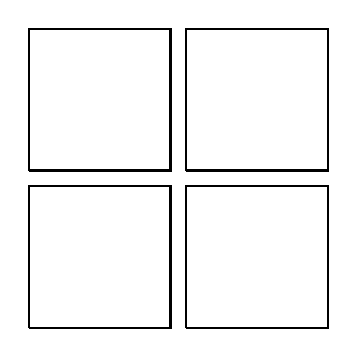
\begin{tikzpicture}[scale=2]
%\draw [thick] (-0.05,-0.05)--(-0.05,2.05)--(2.05,2.05)--(2.05,-0.05)--(-0.05,-0.05);
\draw [thick] (0.05,0.05)--(0.95,0.05)--(0.95,0.95)--(0.05,0.95)--(0.05,0.05);
\draw [thick] (1.05,0.05)--(1.95,0.05)--(1.95,0.95)--(1.05,0.95)--(1.05,0.05);
\draw [thick] (1.05,1.05)--(1.95,1.05)--(1.95,1.95)--(1.05,1.95)--(1.05,1.05);
\draw [thick] (0.05,1.05)--(0.95,1.05)--(0.95,1.95)--(0.05,1.95)--(0.05,1.05);
%\node (1) at (1,1) {$D$};
\end{tikzpicture}
\end{center}

Then we can measure the curl around each of those four regions, which is the counter clockwise circulation.

\begin{center}
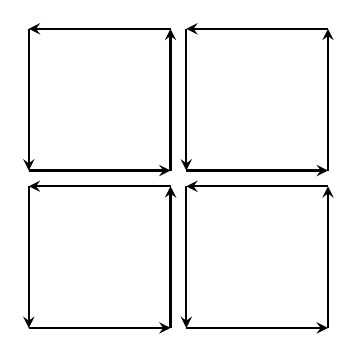
\begin{tikzpicture}[scale=2]
%\draw [thick] (0,0)--(0,2)--(2,2)--(2,0)--(0,0);
%\draw [thick] (-0.05,-0.05)--(-0.05,2.05)--(2.05,2.05)--(2.05,-0.05)--(-0.05,-0.05);
\draw [-stealth,thick](0.05,0.05)--(0.95,0.05);
\draw [-stealth,thick](0.95,0.05)--(0.95,0.95);
\draw [-stealth,thick](0.95,0.95)--(0.05,0.95);
\draw [-stealth,thick](0.05,0.95)--(0.05,0.05);

\draw [-stealth,thick](1.05,0.05)--(1.95,0.05);
\draw [-stealth,thick](1.95,0.05)--(1.95,0.95);
\draw [-stealth,thick](1.95,0.95)--(1.05,0.95);
\draw [-stealth,thick](1.05,0.95)--(1.05,0.05);

\draw [-stealth,thick](1.05,1.05)--(1.95,1.05);
\draw [-stealth,thick](1.95,1.05)--(1.95,1.95);
\draw [-stealth,thick](1.95,1.95)--(1.05,1.95);
\draw [-stealth,thick](1.05,1.95)--(1.05,1.05);

\draw [-stealth,thick](0.05,1.05)--(0.95,1.05);
\draw [-stealth,thick](0.95,1.05)--(0.95,1.95);
\draw [-stealth,thick](0.95,1.95)--(0.05,1.95);
\draw [-stealth,thick](0.05,1.95)--(0.05,1.05);
%\node (1) at (1,1) {$D$};
\end{tikzpicture}
\end{center}

We can continue breaking the regions down into smaller and smaller subregions if we want.

\begin{center}
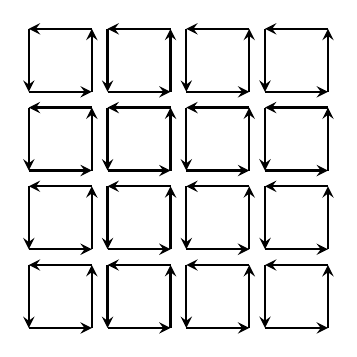
\begin{tikzpicture}[scale=2]
%\draw [thick] (0,0)--(0,2)--(2,2)--(2,0)--(0,0);
%\draw [thick] (-0.05,-0.05)--(-0.05,2.05)--(2.05,2.05)--(2.05,-0.05)--(-0.05,-0.05);
\draw [-stealth,thick](0.05,0.05)--(0.45,0.05);
\draw [-stealth,thick](0.45,0.05)--(0.45,0.45);
\draw [-stealth,thick](0.45,0.45)--(0.05,0.45);
\draw [-stealth,thick](0.05,0.45)--(0.05,0.05);

\draw [-stealth,thick](0.05,0.55)--(0.45,0.55);
\draw [-stealth,thick](0.45,0.55)--(0.45,0.95);
\draw [-stealth,thick](0.45,0.95)--(0.05,0.95);
\draw [-stealth,thick](0.05,0.95)--(0.05,0.55);

\draw [-stealth,thick](0.55,0.05)--(0.95,0.05);
\draw [-stealth,thick](0.95,0.05)--(0.95,0.45);
\draw [-stealth,thick](0.95,0.45)--(0.55,0.45);
\draw [-stealth,thick](0.55,0.45)--(0.55,0.05);

\draw [-stealth,thick](0.55,0.55)--(0.95,0.55);
\draw [-stealth,thick](0.95,0.55)--(0.95,0.95);
\draw [-stealth,thick](0.95,0.95)--(0.55,0.95);
\draw [-stealth,thick](0.55,0.95)--(0.55,0.55);


\draw [-stealth,thick](1.05,0.05)--(1.45,0.05);
\draw [-stealth,thick](1.45,0.05)--(1.45,0.45);
\draw [-stealth,thick](1.45,0.45)--(1.05,0.45);
\draw [-stealth,thick](1.05,0.45)--(1.05,0.05);

\draw [-stealth,thick](1.05,0.55)--(1.45,0.55);
\draw [-stealth,thick](1.45,0.55)--(1.45,0.95);
\draw [-stealth,thick](1.45,0.95)--(1.05,0.95);
\draw [-stealth,thick](1.05,0.95)--(1.05,0.55);

\draw [-stealth,thick](1.55,0.05)--(1.95,0.05);
\draw [-stealth,thick](1.95,0.05)--(1.95,0.45);
\draw [-stealth,thick](1.95,0.45)--(1.55,0.45);
\draw [-stealth,thick](1.55,0.45)--(1.55,0.05);

\draw [-stealth,thick](1.55,0.55)--(1.95,0.55);
\draw [-stealth,thick](1.95,0.55)--(1.95,0.95);
\draw [-stealth,thick](1.95,0.95)--(1.55,0.95);
\draw [-stealth,thick](1.55,0.95)--(1.55,0.55);


\draw [-stealth,thick](0.05,1.05)--(0.45,1.05);
\draw [-stealth,thick](0.45,1.05)--(0.45,1.45);
\draw [-stealth,thick](0.45,1.45)--(0.05,1.45);
\draw [-stealth,thick](0.05,1.45)--(0.05,1.05);

\draw [-stealth,thick](0.05,1.55)--(0.45,1.55);
\draw [-stealth,thick](0.45,1.55)--(0.45,1.95);
\draw [-stealth,thick](0.45,1.95)--(0.05,1.95);
\draw [-stealth,thick](0.05,1.95)--(0.05,1.55);

\draw [-stealth,thick](0.55,1.05)--(0.95,1.05);
\draw [-stealth,thick](0.95,1.05)--(0.95,1.45);
\draw [-stealth,thick](0.95,1.45)--(0.55,1.45);
\draw [-stealth,thick](0.55,1.45)--(0.55,1.05);

\draw [-stealth,thick](0.55,1.55)--(0.95,1.55);
\draw [-stealth,thick](0.95,1.55)--(0.95,1.95);
\draw [-stealth,thick](0.95,1.95)--(0.55,1.95);
\draw [-stealth,thick](0.55,1.95)--(0.55,1.55);


\draw [-stealth,thick](1.05,1.05)--(1.45,1.05);
\draw [-stealth,thick](1.45,1.05)--(1.45,1.45);
\draw [-stealth,thick](1.45,1.45)--(1.05,1.45);
\draw [-stealth,thick](1.05,1.45)--(1.05,1.05);

\draw [-stealth,thick](1.05,1.55)--(1.45,1.55);
\draw [-stealth,thick](1.45,1.55)--(1.45,1.95);
\draw [-stealth,thick](1.45,1.95)--(1.05,1.95);
\draw [-stealth,thick](1.05,1.95)--(1.05,1.55);

\draw [-stealth,thick](1.55,1.05)--(1.95,1.05);
\draw [-stealth,thick](1.95,1.05)--(1.95,1.45);
\draw [-stealth,thick](1.95,1.45)--(1.55,1.45);
\draw [-stealth,thick](1.55,1.45)--(1.55,1.05);

\draw [-stealth,thick](1.55,1.55)--(1.95,1.55);
\draw [-stealth,thick](1.95,1.55)--(1.95,1.95);
\draw [-stealth,thick](1.95,1.95)--(1.55,1.95);
\draw [-stealth,thick](1.55,1.95)--(1.55,1.55);

%\node (1) at (1,1) {$D$};
\end{tikzpicture}
\end{center}

We can continue doing this until we have infinitesimally small subregions. Then when we look at the curl on two adjacent subregions we see that the shared edge of the subregion has equal and opposite rotational tendency. When accumulating the total rotation, these edges cancel, leaving us with just the rotational tendency about the border of the pair.

\begin{center}
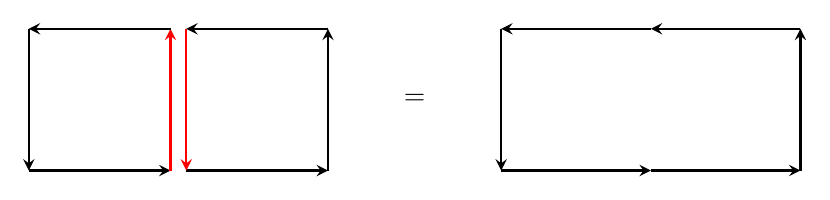
\begin{tikzpicture}[scale=2]
%\draw [thick] (0,0)--(0,2)--(2,2)--(2,0)--(0,0);
%\draw [thick] (-0.05,-0.05)--(-0.05,2.05)--(2.05,2.05)--(2.05,-0.05)--(-0.05,-0.05);
\draw [-stealth,thick](0.05,0.05)--(0.95,0.05);
\draw [-stealth,thick,red](0.95,0.05)--(0.95,0.95);
\draw [-stealth,thick](0.95,0.95)--(0.05,0.95);
\draw [-stealth,thick](0.05,0.95)--(0.05,0.05);

\draw [-stealth,thick](1.05,0.05)--(1.95,0.05);
\draw [-stealth,thick](1.95,0.05)--(1.95,0.95);
\draw [-stealth,thick](1.95,0.95)--(1.05,0.95);
\draw [-stealth,thick,red](1.05,0.95)--(1.05,0.05);
%\node (1) at (1,1) {$D$};
\node(=) at (2.5,0.5) {$=$};

\draw [-stealth,thick](3.05,0.05)--(4,0.05);
%\draw [-stealth,thick](3.95,0.05)--(3.95,0.95);
\draw [-stealth,thick](4,0.95)--(3.05,0.95);
\draw [-stealth,thick](3.05,0.95)--(3.05,0.05);

\draw [-stealth,thick](4,0.05)--(4.95,0.05);
\draw [-stealth,thick](4.95,0.05)--(4.95,0.95);
\draw [-stealth,thick](4.95,0.95)--(4,0.95);
%\draw [-stealth,thick](4.05,0.95)--(4.05,0.05);
\end{tikzpicture}
\end{center}

We can expand this out and cancel equal and opposite pairs as necessary.

\begin{center}
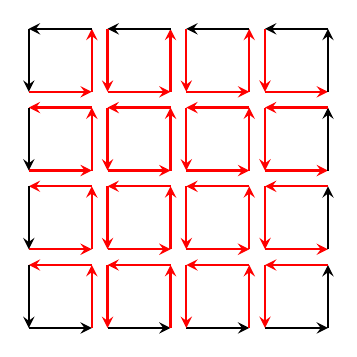
\begin{tikzpicture}[scale=2]
%\draw [thick] (0,0)--(0,2)--(2,2)--(2,0)--(0,0);
%\draw [thick] (-0.05,-0.05)--(-0.05,2.05)--(2.05,2.05)--(2.05,-0.05)--(-0.05,-0.05);
\draw [-stealth,thick](0.05,0.05)--(0.45,0.05);
\draw [-stealth,thick,red](0.45,0.05)--(0.45,0.45);
\draw [-stealth,thick,red](0.45,0.45)--(0.05,0.45);
\draw [-stealth,thick](0.05,0.45)--(0.05,0.05);

\draw [-stealth,thick,red](0.05,0.55)--(0.45,0.55);
\draw [-stealth,thick,red](0.45,0.55)--(0.45,0.95);
\draw [-stealth,thick,red](0.45,0.95)--(0.05,0.95);
\draw [-stealth,thick](0.05,0.95)--(0.05,0.55);

\draw [-stealth,thick](0.55,0.05)--(0.95,0.05);
\draw [-stealth,thick,red](0.95,0.05)--(0.95,0.45);
\draw [-stealth,thick,red](0.95,0.45)--(0.55,0.45);
\draw [-stealth,thick,red](0.55,0.45)--(0.55,0.05);

\draw [-stealth,thick,red](0.55,0.55)--(0.95,0.55);
\draw [-stealth,thick,red](0.95,0.55)--(0.95,0.95);
\draw [-stealth,thick,red](0.95,0.95)--(0.55,0.95);
\draw [-stealth,thick,red](0.55,0.95)--(0.55,0.55);


\draw [-stealth,thick](1.05,0.05)--(1.45,0.05);
\draw [-stealth,thick,red](1.45,0.05)--(1.45,0.45);
\draw [-stealth,thick,red](1.45,0.45)--(1.05,0.45);
\draw [-stealth,thick,red](1.05,0.45)--(1.05,0.05);

\draw [-stealth,thick,red](1.05,0.55)--(1.45,0.55);
\draw [-stealth,thick,red](1.45,0.55)--(1.45,0.95);
\draw [-stealth,thick,red](1.45,0.95)--(1.05,0.95);
\draw [-stealth,thick,red](1.05,0.95)--(1.05,0.55);

\draw [-stealth,thick](1.55,0.05)--(1.95,0.05);
\draw [-stealth,thick](1.95,0.05)--(1.95,0.45);
\draw [-stealth,thick,red](1.95,0.45)--(1.55,0.45);
\draw [-stealth,thick,red](1.55,0.45)--(1.55,0.05);

\draw [-stealth,thick,red](1.55,0.55)--(1.95,0.55);
\draw [-stealth,thick](1.95,0.55)--(1.95,0.95);
\draw [-stealth,thick,red](1.95,0.95)--(1.55,0.95);
\draw [-stealth,thick,red](1.55,0.95)--(1.55,0.55);


\draw [-stealth,thick,red](0.05,1.05)--(0.45,1.05);
\draw [-stealth,thick,red](0.45,1.05)--(0.45,1.45);
\draw [-stealth,thick,red](0.45,1.45)--(0.05,1.45);
\draw [-stealth,thick](0.05,1.45)--(0.05,1.05);

\draw [-stealth,thick,red](0.05,1.55)--(0.45,1.55);
\draw [-stealth,thick,red](0.45,1.55)--(0.45,1.95);
\draw [-stealth,thick](0.45,1.95)--(0.05,1.95);
\draw [-stealth,thick](0.05,1.95)--(0.05,1.55);

\draw [-stealth,thick,red](0.55,1.05)--(0.95,1.05);
\draw [-stealth,thick,red](0.95,1.05)--(0.95,1.45);
\draw [-stealth,thick,red](0.95,1.45)--(0.55,1.45);
\draw [-stealth,thick,red](0.55,1.45)--(0.55,1.05);

\draw [-stealth,thick,red](0.55,1.55)--(0.95,1.55);
\draw [-stealth,thick,red](0.95,1.55)--(0.95,1.95);
\draw [-stealth,thick](0.95,1.95)--(0.55,1.95);
\draw [-stealth,thick,red](0.55,1.95)--(0.55,1.55);


\draw [-stealth,thick,red](1.05,1.05)--(1.45,1.05);
\draw [-stealth,thick,red](1.45,1.05)--(1.45,1.45);
\draw [-stealth,thick,red](1.45,1.45)--(1.05,1.45);
\draw [-stealth,thick,red](1.05,1.45)--(1.05,1.05);

\draw [-stealth,thick,red](1.05,1.55)--(1.45,1.55);
\draw [-stealth,thick,red](1.45,1.55)--(1.45,1.95);
\draw [-stealth,thick](1.45,1.95)--(1.05,1.95);
\draw [-stealth,thick,red](1.05,1.95)--(1.05,1.55);

\draw [-stealth,thick,red](1.55,1.05)--(1.95,1.05);
\draw [-stealth,thick](1.95,1.05)--(1.95,1.45);
\draw [-stealth,thick,red](1.95,1.45)--(1.55,1.45);
\draw [-stealth,thick,red](1.55,1.45)--(1.55,1.05);

\draw [-stealth,thick,red](1.55,1.55)--(1.95,1.55);
\draw [-stealth,thick](1.95,1.55)--(1.95,1.95);
\draw [-stealth,thick](1.95,1.95)--(1.55,1.95);
\draw [-stealth,thick,red](1.55,1.95)--(1.55,1.55);

%\node (1) at (1,1) {$D$};
\end{tikzpicture}
\end{center}

After cancelling, we're left with just the circulation about the boundary.

\begin{center}
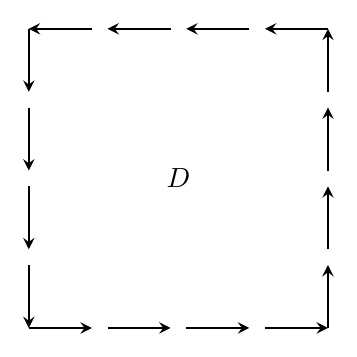
\begin{tikzpicture}[scale=2]
%\draw [thick] (0,0)--(0,2)--(2,2)--(2,0)--(0,0);
%\draw [thick] (-0.05,-0.05)--(-0.05,2.05)--(2.05,2.05)--(2.05,-0.05)--(-0.05,-0.05);
\draw [-stealth,thick](0.05,0.05)--(0.45,0.05);
%\draw [-stealth,thick,red](0.45,0.05)--(0.45,0.45);
%\draw [-stealth,thick,red](0.45,0.45)--(0.05,0.45);
\draw [-stealth,thick](0.05,0.45)--(0.05,0.05);

%\draw [-stealth,thick,red](0.05,0.55)--(0.45,0.55);
%\draw [-stealth,thick,red](0.45,0.55)--(0.45,0.95);
%\draw [-stealth,thick,red](0.45,0.95)--(0.05,0.95);
\draw [-stealth,thick](0.05,0.95)--(0.05,0.55);

\draw [-stealth,thick](0.55,0.05)--(0.95,0.05);
%\draw [-stealth,thick,red](0.95,0.05)--(0.95,0.45);
%\draw [-stealth,thick,red](0.95,0.45)--(0.55,0.45);
%\draw [-stealth,thick,red](0.55,0.45)--(0.55,0.05);

%\draw [-stealth,thick,red](0.55,0.55)--(0.95,0.55);
%\draw [-stealth,thick,red](0.95,0.55)--(0.95,0.95);
%\draw [-stealth,thick,red](0.95,0.95)--(0.55,0.95);
%\draw [-stealth,thick,red](0.55,0.95)--(0.55,0.55);


\draw [-stealth,thick](1.05,0.05)--(1.45,0.05);
%\draw [-stealth,thick,red](1.45,0.05)--(1.45,0.45);
%\draw [-stealth,thick,red](1.45,0.45)--(1.05,0.45);
%\draw [-stealth,thick,red](1.05,0.45)--(1.05,0.05);

%\draw [-stealth,thick,red](1.05,0.55)--(1.45,0.55);
%\draw [-stealth,thick,red](1.45,0.55)--(1.45,0.95);
%\draw [-stealth,thick,red](1.45,0.95)--(1.05,0.95);
%\draw [-stealth,thick,red](1.05,0.95)--(1.05,0.55);

\draw [-stealth,thick](1.55,0.05)--(1.95,0.05);
\draw [-stealth,thick](1.95,0.05)--(1.95,0.45);
%\draw [-stealth,thick,red](1.95,0.45)--(1.55,0.45);
%\draw [-stealth,thick,red](1.55,0.45)--(1.55,0.05);

%\draw [-stealth,thick,red](1.55,0.55)--(1.95,0.55);
\draw [-stealth,thick](1.95,0.55)--(1.95,0.95);
%\draw [-stealth,thick,red](1.95,0.95)--(1.55,0.95);
%\draw [-stealth,thick,red](1.55,0.95)--(1.55,0.55);


%\draw [-stealth,thick,red](0.05,1.05)--(0.45,1.05);
%\draw [-stealth,thick,red](0.45,1.05)--(0.45,1.45);
%\draw [-stealth,thick,red](0.45,1.45)--(0.05,1.45);
\draw [-stealth,thick](0.05,1.45)--(0.05,1.05);

%\draw [-stealth,thick,red](0.05,1.55)--(0.45,1.55);
%\draw [-stealth,thick,red](0.45,1.55)--(0.45,1.95);
\draw [-stealth,thick](0.45,1.95)--(0.05,1.95);
\draw [-stealth,thick](0.05,1.95)--(0.05,1.55);

%\draw [-stealth,thick,red](0.55,1.05)--(0.95,1.05);
%\draw [-stealth,thick,red](0.95,1.05)--(0.95,1.45);
%\draw [-stealth,thick,red](0.95,1.45)--(0.55,1.45);
%\draw [-stealth,thick,red](0.55,1.45)--(0.55,1.05);

%\draw [-stealth,thick,red](0.55,1.55)--(0.95,1.55);
%\draw [-stealth,thick,red](0.95,1.55)--(0.95,1.95);
\draw [-stealth,thick](0.95,1.95)--(0.55,1.95);
%\draw [-stealth,thick,red](0.55,1.95)--(0.55,1.55);


%\draw [-stealth,thick,red](1.05,1.05)--(1.45,1.05);
%\draw [-stealth,thick,red](1.45,1.05)--(1.45,1.45);
%\draw [-stealth,thick,red](1.45,1.45)--(1.05,1.45);
%\draw [-stealth,thick,red](1.05,1.45)--(1.05,1.05);

%\draw [-stealth,thick,red](1.05,1.55)--(1.45,1.55);
%\draw [-stealth,thick,red](1.45,1.55)--(1.45,1.95);
\draw [-stealth,thick](1.45,1.95)--(1.05,1.95);
%\draw [-stealth,thick,red](1.05,1.95)--(1.05,1.55);

%\draw [-stealth,thick,red](1.55,1.05)--(1.95,1.05);
\draw [-stealth,thick](1.95,1.05)--(1.95,1.45);
%\draw [-stealth,thick,red](1.95,1.45)--(1.55,1.45);
%\draw [-stealth,thick,red](1.55,1.45)--(1.55,1.05);

%\draw [-stealth,thick,red](1.55,1.55)--(1.95,1.55);
\draw [-stealth,thick](1.95,1.55)--(1.95,1.95);
\draw [-stealth,thick](1.95,1.95)--(1.55,1.95);
%\draw [-stealth,thick,red](1.55,1.95)--(1.55,1.55);

\node (1) at (1,1) {$D$};
\end{tikzpicture}
\end{center}

This is exactly the line integral, $$\int_{C}\vcF \ dr. $$

Green's theorem is a good example of a theorem where both directions are useful. For example, sometimes you have a line integral on a curve that would require an annoying parameterization, but the region that's enclosed is actually quite easy to describe.

\begin{example}{An Annoying Line Integral}
Let $\vcF=\bmat{xy\\-x}$. Let $C$ be the positively oriented rectangle with a corner at $(0,0)$ and $(1,1)$.

\begin{center}
\begin{tikzpicture}[scale=2]
\draw (-0.5,0)--(1.5,0);
\draw (0,-0.5)--(0,1.5);
\draw [-stealth,thick] (0,0)--(1,0);
\draw [-stealth,thick] (1,0)--(1,1);
\draw [-stealth,thick] (1,1)--(0,1);
\draw [-stealth,thick] (0,1)--(0,0);
\draw [gray] (1,0.05)--(1,-0.05);
%\draw [gray] (-1,0.05)--(-1,-0.05);
%\draw [gray] (2,0.05)--(2,-0.05);
\draw [gray] (0.05,1)--(-0.05,1);
%\draw [gray] (0.05,2)--(-0.05,2);
%\draw [gray] (0.05,-1)--(-0.05,-1);
\end{tikzpicture}\\
The positively oriented path, $C$.
\end{center}

Suppose we wanted to evaluate $$\int_C \vcF \ dr. $$ 

To evaluate this line integral, it would be necessary to actually parameterize our line integrals over four separate sections. That is, we could define:
\begin{align*}
C_1=&\left\{\vcr_1(t):\ \vcr_1(t)=\bmat{t\\0}, \ 0\leq t\leq 1 \right\}\\
C_2=&\left\{\vcr_2(t):\ \vcr_2(t)=\bmat{1\\t-1}, \ 1\leq t\leq 2 \right\}\\
C_3=&\left\{\vcr_3(t):\ \vcr_3(t)=\bmat{3-t\\1}, \ 2\leq t\leq 3 \right\}\\
C_4=&\left\{\vcr_4(t):\ \vcr_4(t)=\bmat{0\\4-t}, \ 3\leq t\leq 4 \right\}
\end{align*}
Then we could evaluate:
$$\int_C \vcF \ dr=\int_{C_1} \vcF \ dr+\int_{C_2} \vcF \ dr+\int_{C_3} \vcF \ dr+\int_{C_4} \vcF \ dr.$$
\end{example}

\begin{exercise}{A Piecewise Line Integral}
Find $$\int_C \vcF \ dr=\int_{C_1} \vcF \ dr+\int_{C_2} \vcF \ dr+\int_{C_3} \vcF \ dr+\int_{C_4} \vcF \ dr$$ using the parameterization from the example above.
\end{exercise}

\begin{exercise}{Green's Theorem to the Rescue}
Use Green's theorem to rewrite the integral from the previous problem as a double integral, then solve.
\end{exercise}

\begin{exercise}{Nephroid, Area by Line Integral}
If you roll a circle of radius 1 around a circle of radius 2, then fix a point on the circle of radius 1, that point traces out the curve known as the \textit{nephroid.}

\vspace{1em}

\begin{center}
\includegraphics[scale=0.25]{Figures/nephroid}\\
Visit \href{https://www.desmos.com/calculator/a8o5rvqufn}{Desmos} to see the nephroid traced out.
\end{center}

\vspace{1em}

Call the region enclosed by the nephroid $R$. Then we could compute the area of the nephroid as $$\iint_R 1 \ dA.$$
Unfortunately, parameterizing the nephroid as a function is quite annoying, so instead we will try to apply Green's Theorem to evaluate the area using a line integral. Let $$\vcF=\bmat{0\\x}, $$ a vector field chosen specifically because it has a curl of $1$. Then $$\iint_R 1 \ dA =\iint_R \curl\vcF \ dA.$$ With this clever choice of $\vcF$, Green's Theorem applies, which means that we can evaluate this area using a \textbf{line integral.}

\vspace{1em}

Use the fact that the nephroid curve can be parameterized as $$\vcr(t)=\bmat{3\cos(t)-\cos(3t)\\3\sin(t)-\sin(3t)},\ 0\leq t\leq 2\pi$$ and Green's Theorem to verify that the area of the nephroid is $12\pi$. Note that the resulting integral you get here can be solved using the triple angle identities:
\begin{align*}
\sin(3\theta)&=3\sin(\theta)-4\sin^3(\theta),\\
\cos(3\theta)&=4\cos^3(\theta)-3\cos(\theta).
\end{align*}
\end{exercise}

\begin{exercise}{Sine Flowers}
Consider the region $R$ inside the polar function $r=\sin(2\theta)$, where $0\leq\theta\leq \frac{\pi}{2}$. Find the area of $R$ in two ways.

\vspace{1em}
\begin{enumerate}
\item Using a double integral, $$\iint_R 1\ dA.$$ Hint: You probably want to convert to polar coordinates.
\vspace{1em}
\item Using a line integral $$\int_C \vcF\ dr $$ where $$\vcF=\bmat{0\\x}\text{ and }C=\vcr(t)=\bmat{2\sin(t)\cos^2(t)\\2\sin^2(t)\cos(t)},\ 0\leq t\leq \frac{\pi}{2}.$$ This integral can be done by hand, but is relatively long, so feel free to use a CAS to solve.
\end{enumerate}
\end{exercise}